
\documentclass[../../../all/physics-standard_answers_all.tex]{subfiles}

\graphicspath{{../../../../figures/}}

\begin{document}

\setlength{\abovedisplayskip}{2mm}
\setlength{\belowdisplayskip}{1mm}

\begin{enumerate}

    \item この直線を中心軸とする円柱（半径$r$，高さ$\ell$）を考える．
        \uline{$0<r<a$}の領域では，円筒の内部には電気力線は無いことに留意して，
        %
        \begin{align*}
            E(r) = \uwave{0} \;.
        \end{align*}
        %
        \uline{$r>a$}の領域では，電気力線は側面を垂直に貫くから，
        %
        \begin{align*}
            E(r)
            = \frac{2 \pi a \ell \sigma / \varepsilon_0}{2\pi r \ell}
            = \uwave{\frac{a \sigma}{\varepsilon_0 r}} \;.
        \end{align*}

    \item 　
        \par {\centering
            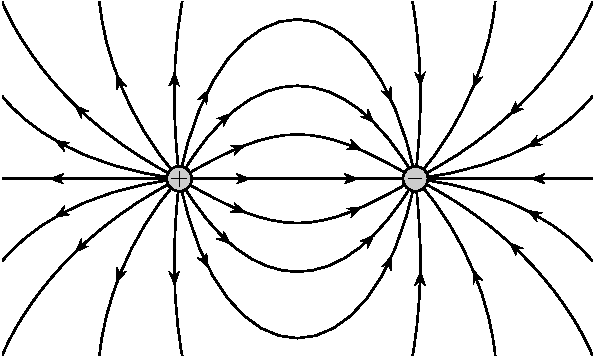
\includegraphics[width=0.9\linewidth]
            {a_electric-field_08_02/physics-standard_answers_electric-field_08_02_tikz.pdf}
        \par}
        \vspace{0.2\baselineskip}

\end{enumerate}

\end{document}
